\documentclass[12pt,a4paper]{article}
\usepackage[utf8]{vietnam}
\usepackage{amsmath}
\usepackage{amssymb}
\usepackage{makeidx}
\usepackage{graphicx}
\usepackage{tabularx, booktabs}

\usepackage[table,xcdraw]{xcolor}
\usepackage[margin=2cm]{geometry}
\usepackage{caption}
\usepackage{subcaption}

\usepackage{hyperref}
\hypersetup{
	colorlinks=true,
	linkcolor=blue,
	filecolor=magenta,      
	urlcolor=cyan,
	pdfpagemode=FullScreen,
}

\usepackage{fancyhdr}
\pagestyle{fancy}
\fancyhf{}
\renewcommand{\headrulewidth}{0pt}
\lhead{\textit{\small HCMC University of Technology and Education}}
\fancyfoot[C]{\thepage}

\usepackage{titlesec}
\titleformat*{\section}{\fontsize{13}{01}\bfseries}
\titleformat*{\subsection}{\fontsize{12}{01}\bfseries}

\title{
	\centering\normalsize  
	\vspace{-0.7in}
	\colorbox{black}{\parbox{\linewidth}{\textcolor{white}{\hfill\HCMUTE \hfill}}} \\[0.5ex]
	\begin{minipage}{\dimexpr0.5\linewidth-0.5\wlogo}\oriart\end{minipage}%
	\begin{minipage}{\dimexpr0.5\linewidth+0.5\wlogo-6pt}\LOGO \end{minipage}\\[0.5ex]
	\colorbox{black}{\parbox{\linewidth}{\textcolor{white}{\hfill\KHCMUTE\hfill}}}\\[1ex]
	\titleofArt
}
\newlength{\wlogo}

\author{Nguyễn Trọng Đại\\19146146}
\date{} 
\newcommand{\HCMUTE}{\normalsize\bfseries\itshape HCMC University of Technology and Education}
\newcommand{\KHCMUTE}{\normalsize\bfseries\itshape Khoa Cơ khí Chế tạo máy}
\newcommand{\oriart}{
\includegraphics[width=\wlogo]{Images/githubQR.eps} 
\includegraphics[width=\wlogo]{Images/githubQR.eps}} 
\setlength{\wlogo}{2.15cm}
\newcommand{\LOGO}{
\includegraphics[width=\wlogo]{Images/logo.png}}
\newcommand{\titleofArt}{\textbf{ \large ỨNG DỤNG CNN NHẬN BIẾT 7 LOẠI BỆNH UNG THƯ DA QUA HÌNH ẢNH VÀ VIDEO}}

\begin{document}
	\maketitle
	\fancypagestyle{Initial}{%
		%\addtolength\topmargin{-0.7in}
		\fancyhead{}
	}
	\thispagestyle{Initial}
	\noindent
	\rule{\textwidth}{0.4pt}
	
	%%%%%%%%%%%%%%%%%%%%%%%%%%%%%%%%%%%%%%%%%%%%%%%%%%%
	\section*{Tóm tắt}
	
	\textit{Cơ sở và mục tiêu của đề tài:} Ung thư da hay da bị tổn thương có dấu hiệu là những đóm đỏ trên tay, mụn nhỏ tưởng chừng như nốt ruồi hay những dấu hiệu được coi là bất thường có trên da người so với các khu vực xung quanh của da. Một vài dấu hiệu có thể vô hại như những vết xước nhỏ hoặc có thể nghiêm trọng hơn là ung thư da. Và để nhận biết được những vùng da bị tổn thương này, khám ở các bệnh viện thường khá là đắt đỏ vì thế trong bài báo này tôi sẽ trình bày về việc ứng dụng mạng CNN để sàn lọc 7 loại bệnh về ung thư da.\\
	
	\noindent
	\textit{Phương pháp:} Trong bài báo này tôi xây dựng mạng CNN có khả năng phân loại được 7 loại ung thư da với độ chính xác chấp nhận được, và tập dữ liệu mà tôi sử dụng là HAM10000. Và tôi sử dụng Framework Flask kết hợp cùng TensorflowJS để xây dựng ứng dụng nhận diện thông qua Website.\\
	
	\noindent
	\textit{Kết quả:} Tôi đã xây dựng được mạng CNN để sàn lọc với kết quả ..., recall ..., predict,... . Cùng với đó tôi đã xây dựng hệ thống Webserver nhận diện realtime trực tuyến tại đia chỉ: \href{https://skincancer.svute.com}{https://skincancer.svute.com}.\\
	
	\noindent
	\textit{Kết luận:} Hi vọng với sản phẩm này có thể giúp người có nghi ngờ về bệnh của mình có thể sử dụng để sàn lọc trước khi đến bệnh viện khám. Và giúp bác sĩ có thể sàn lọc bệnh nhân và giảm chi phí khám bệnh.
	
	\hfill \break
	\noindent
	\rule{\textwidth}{0.4pt}
	%%%%%%%%%%%%%%%%%%%%%%%%%%%%%%%%%%%%%%%%%%%%%%%%%%
	
	\section{Giới thiệu}
	Ung thư da là một trong những bệnh rất phổ biến trên thế giới, cụ thể ở Mỹ mỗi năm có hơn 5 triệu ca mắc phải, mỗi năm có hơn 9000 người chết vì ung thư da. Điều trị ung thư da tốn chi phí rất lớn. Vì thế ung thư da trở thành một mối đe doạ lớn đến với cộng đồng. Tỉ lệ mắc ung thư da đã tăng lên hằng năm là một điều rất đáng báo động.\\
	
	\noindent
	Trước đây ung thư da được chuẩn đoán lâm sàng và không có bất kỳ sự hỗ trợ nào, và được đánh giá bằng mức độ kinh nghiệm của người bác sĩ. Điều này dẫn đến thiếu sự chính xác trong chuẩn đoán. Trong những năm gần đây thì kỹ thuật nội soi đã bắt đầu phát triển và được ứng dụng vào  trong việc chẩn đoán bệnh của bác sĩ.\\
	
	\noindent
	Với những lý do trên cùng với sự phát triển của kỹ thuật nội soi đã cho chúng ta một tập dữ liệu về tổn thương da, cùng với đó là sự phát triển của AI và Deep learning chúng ta có thể tạo ra một mô hình chẩn đoán lâm sàng. Vì thế trong bài báo này tôi sẽ ứng dụng "mạng thần kinh tích chập" - CNN nhầm mục đích tạo ra một mô hình chẩn đoán và tạo ra một môi trường Realtime cho mọi người có thể vào và chẩn đoán lâm sàng.
	
	%%%%%%%%%%%%%%%%%%%%%%%%%%%%%%%%%%%%%%%%%%%%%%%
	
	\section{Phương pháp}
	
	Trong đề tài này tôi sẽ trải qua 7 bước theo quy trình như hình dưới đây. Đầu tiên là tôi sử dụng tập dữ liệu HAM10000 sẽ được trình bày ở phần sau, tôi sẽ trải qua các bước xử lý dữ liệu, xử lý mất cân bằng trong tập dữ liệu, khi dữ liệu đã ổn định tôi xây dựng cấu trúc mạng CNN thực hiện việc training và turning để cho ra model tốt nhất có thể và triển khai realtime lên Website với Framework Flask.
	
	\begin{figure}[h!]
		\centering
		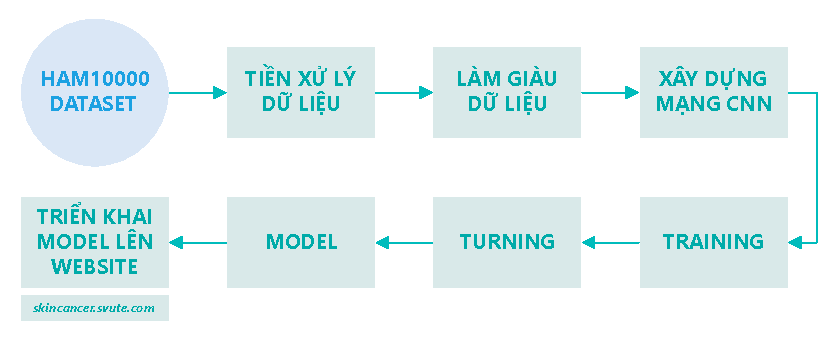
\includegraphics[width=0.8\linewidth]{./images/quatrinh.eps}
		\caption{Các bước thực hiện đề tài}
		\label{fig:quatrinh}
	\end{figure}
	
	\subsection{Tập dữ liệu HAM10000}
	
	HAM10000 là tập dữ liệu được sử dụng trong đề tài này là bộ dữ liệu được công khai bởi đại học Hardvard. Bộ dữ liệu bao gồm 10015 ảnh soi da để phục vụ tạo ra một tiêu chuẩn trong việc chẩn đoán các bệnh về tổn thương da.Tập dữ liệu HAM10000 được sử dụng trong cuộc thi ISIC 2018, trong tập dữ liệu có 7 lớp và 7 lớp này là 7 loại bệnh về tổn thương da cụ thể ở bảng dưới đây.\\
	
	
	\begin{figure}[h!]
		\centering
		\begin{subfigure}[b]{0.3\linewidth}
			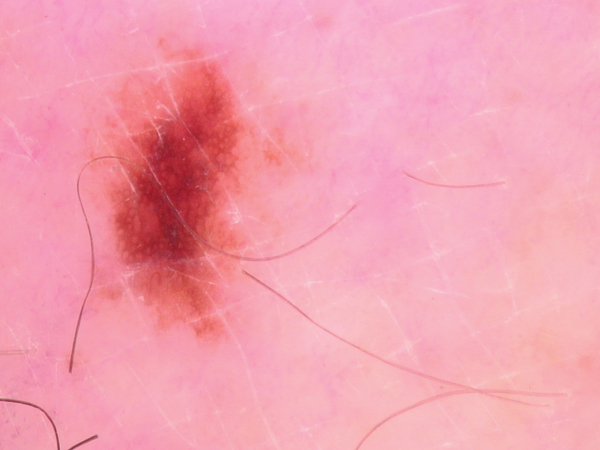
\includegraphics[width=\linewidth]{./images/nv.jpg}
			\caption{Melanocytic nevi.}
		\end{subfigure}
		\begin{subfigure}[b]{0.3\linewidth}
			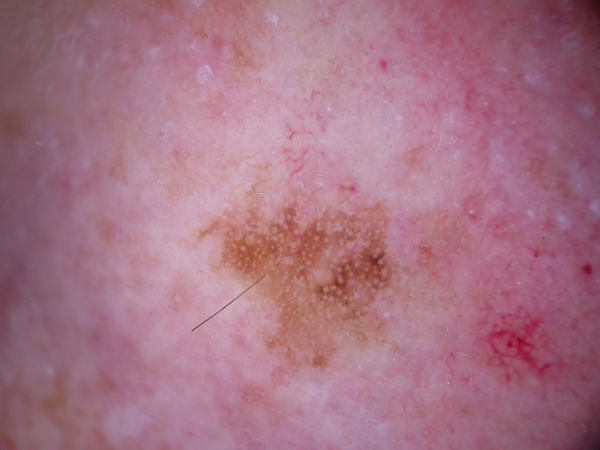
\includegraphics[width=\linewidth]{./images/akiec.jpg}
			\caption{Benign keratosis-like.}
		\end{subfigure}
		\begin{subfigure}[b]{0.3\linewidth}
			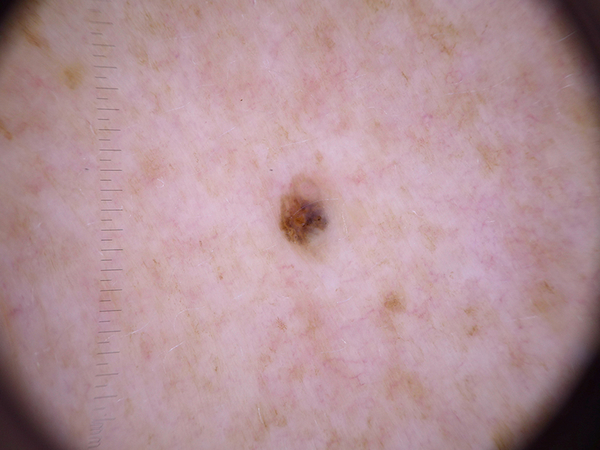
\includegraphics[width=\linewidth]{./images/bkl.jpg}
			\caption{Actinic keratoses.}
		\end{subfigure}
		\caption{Một vài hình ảnh trong tập HAM10000.}
		\label{fig:motvaihinhanh}
	\end{figure}
	
	\begin{center}
		\begin{tabular}{|l|c|}
			\hline
			\rowcolor[HTML]{333333} 
			\multicolumn{1}{|c|}{\cellcolor[HTML]{333333}{\color[HTML]{FFFFFF} \textbf{Loại bệnh}}} & {\color[HTML]{FFFFFF} \textbf{Nhãn}} \\ \hline
			Actinic keratoses                                                                       & 0                                    \\ \hline
			Basal cell carcinoma                                                                    & 1                                    \\ \hline
			Benign keratosis-like lesions                                                           & 2                                    \\ \hline
			Dermatofibroma                                                                          & 3                                    \\ \hline
			Melanocytic nevi                                                                       & 4                                    \\ \hline
			Malignant Melanoma                                                                        & 5                                    \\ \hline
			Vascular lesions                                                                        & 6                                    \\ \hline
		\end{tabular}
	\captionof{table}{Phân lớp các loại bệnh trong tập dữ liệu HAM10000}
	\end{center}

	\noindent
	Tập dữ liệu HAM10000 bị vấn đề về mất cân bằng dữ liệu như hình dưới đây, trong tập dữ liệu này số lượng ảnh về bệnh "Melanocytic nevi" chiếm số lương rất lớn\\	
	
	
	\begin{figure}[h!]
		\centering
		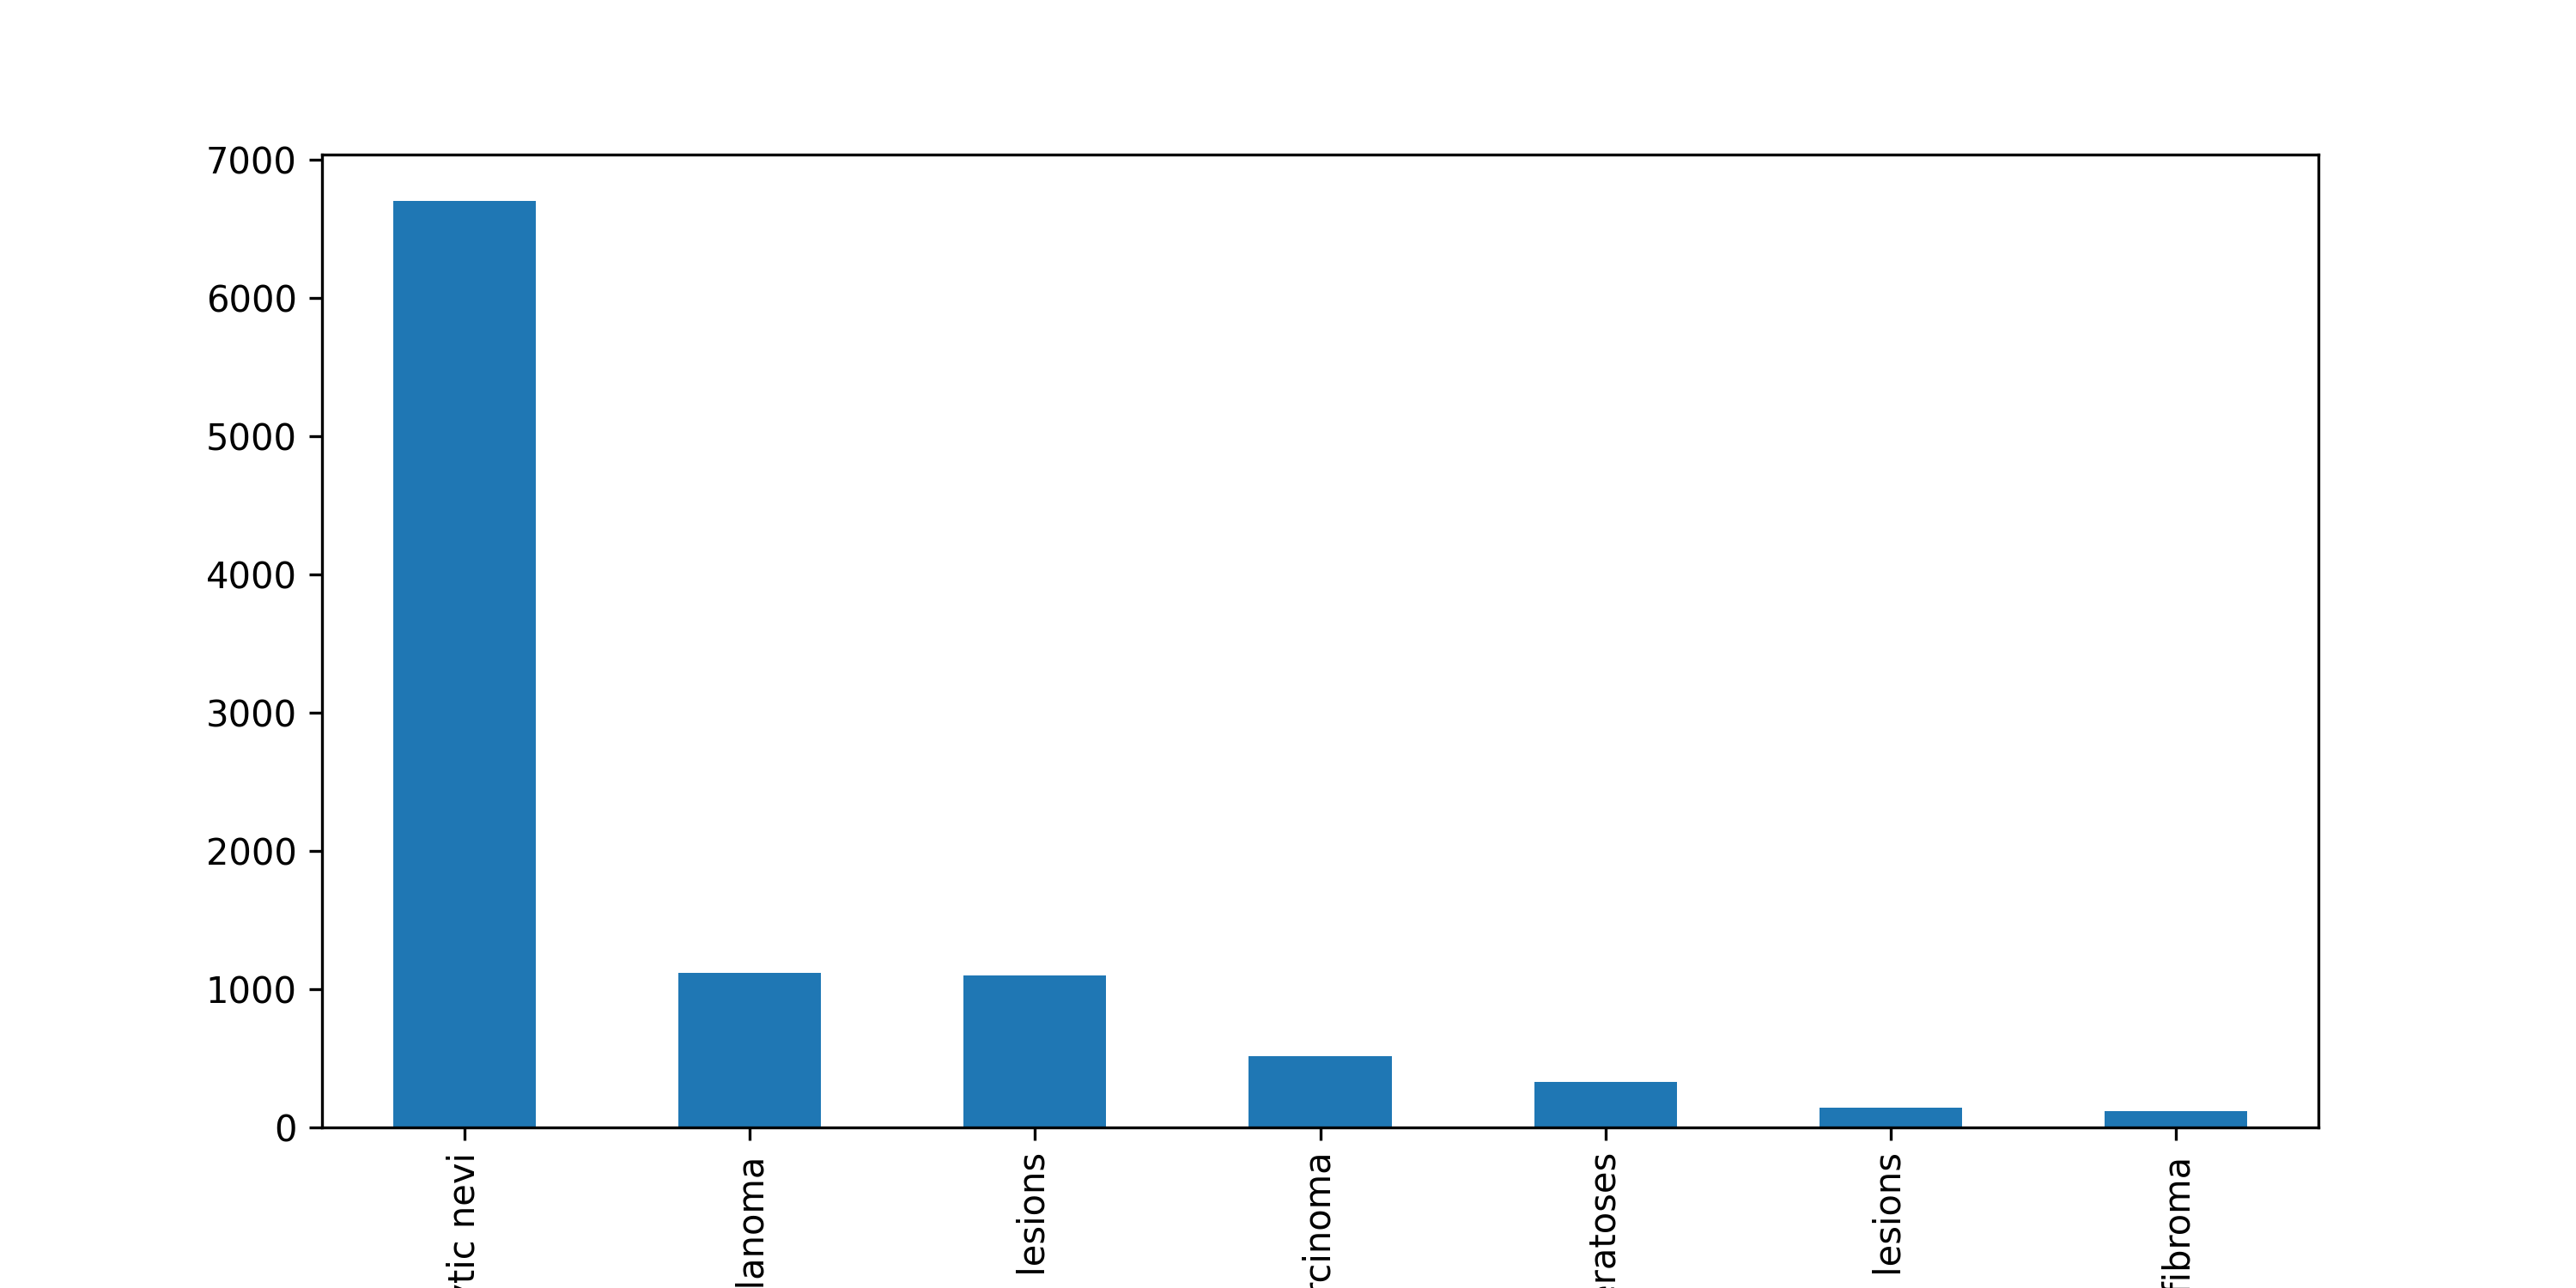
\includegraphics[width=0.5\linewidth]{./images/imbalance.png}
		\caption{Phân bố dữ liệu tập HAM10000.}
		\label{fig:ham10000}
	\end{figure}

	\begin{center}
		\begin{tabular}{|l|c|c|c|c|c|c|c|l|}
			\hline
			\rowcolor[HTML]{000000} 
			{\color[HTML]{FFFFFF} \textbf{Phân lớp}} & {\color[HTML]{FFFFFF} \textbf{0}} & {\color[HTML]{FFFFFF} \textbf{1}} & {\color[HTML]{FFFFFF} \textbf{2}} & {\color[HTML]{FFFFFF} \textbf{3}} & {\color[HTML]{FFFFFF} \textbf{4}} & {\color[HTML]{FFFFFF} \textbf{5}} & {\color[HTML]{FFFFFF} \textbf{6}} & {\color[HTML]{FFFFFF} \textbf{Tổng}} \\ \hline
			\textbf{Số lượng hình ảnh}               & 327                               & 514                               & 1099                              & 115                               & 6705                              & 142                               & 1113                              & 10015                                \\ \hline
		\end{tabular}
	\captionof{table}{Số lượng ảnh trong tập dữ liệu HAM10000}
	\end{center}
	
	\subsection{Tiền xử lý và làm giàu dữ liệu}
	
	Như đã trình bày ở phần trước thì tập HAM10000 bị tình trạng mất cân bằng rất lớn vì thế ở bước tiền xử lý dữ liệu tôi đã sử dụng phương pháp Data Augment nhằm mục đích làm giàu dữ liệu để cân bằng lại tập dữ liệu.\\
	
	\noindent
	Trước khi xử lý dữ liệu mất cân bằng bằng Data Augment thì tôi sẽ áp dụng thêm một phương pháp để tăng độ nhạy của mô hình đối với phân lớp gây mất cân bằng, cụ thể ở đây là lớp bênh \textit{"Melanocytic nevi"}.\\
	
	\begin{center}
		\begin{tabular}{|c|c|c|c|c|c|c|}
			\hline
			\rowcolor[HTML]{000000} 
			{\color[HTML]{FFFFFF} \textbf{akiec}} & {\color[HTML]{FFFFFF} \textbf{bcc}} & {\color[HTML]{FFFFFF} \textbf{bkl}} & {\color[HTML]{FFFFFF} \textbf{df}} & \cellcolor[HTML]{FE0000}{\color[HTML]{FFFFFF} \textbf{nv}} & {\color[HTML]{FFFFFF} \textbf{mel}} & {\color[HTML]{FFFFFF} \textbf{vasc}} \\ \hline
			\textbf{1.0}                          & \textbf{1.0}                        & \textbf{1.0}                        & \textbf{1.0}                       & \cellcolor[HTML]{F8FF00}\textbf{3.5}                       & \textbf{1.0}                        & \textbf{1.0}                         \\ \hline
		\end{tabular}
	\captionof{table}{Tỉ lệ trọng số (class weight) của các phân lớp}
	\end{center}
	
	\noindent
	Việc tăng cường dữ liệu (Data Augment) giúp cho tăng dữ liệu dựa trên các dữ liệu đã có mà không cần phải đi thu thập thêm, một số loại dữ liệu đặc thù rất khó thu thập. Và nó cực kỳ hữu ích cho tập dữ liệu HAM10000 khi tập này bị mất cân bằng rất lớn. Để làm giàu tập dữ liệu bằng việc tăng cường tôi thực hiện các tác động ví dụ như: xoay ảnh, phóng to ảnh, dịch trái, dịch phải ảnh... Và những tham số mà tôi sử dụng được trình bày ở bảng dưới đây.
	
	\begin{center}
		\begin{tabular}{|l|c|l|}
			\hline
			\rowcolor[HTML]{000000} 
			\multicolumn{1}{|c|}{\cellcolor[HTML]{000000}{\color[HTML]{FFFFFF} \textbf{Tham số}}} & {\color[HTML]{FFFFFF} \textbf{Giá trị}} & \multicolumn{1}{c|}{\cellcolor[HTML]{000000}{\color[HTML]{FFFFFF} \textbf{Mô tả}}} \\ \hline
			Rotation range                                                                        & \textbf{180}                            & Cho phép xoay ảnh từ -180 đến 180 độ.                                              \\ \hline
			Width shift range                                                                     & \textbf{0.1}                            & Dịch ảnh ngẫu nhiên theo phương ngang với giá trị là 0.1.                          \\ \hline
			Height shift range                                                                    & \textbf{0.1}                            & Dịch ảnh ngẫu nhiên theo phương dọc với giá trị là 0.1.                            \\ \hline
			Zoom range                                                                            & \textbf{0.1}                            & Phóng to hoặc thu nhỏ ảnh từ giữa ra với giá trị là 0.1.                           \\ \hline
			Horizontal flip                                                                       & \textbf{True}                           & Lật ngẫu nhiên ảnh theo phương ngang.                                              \\ \hline
			Vertical flip                                                                         & \textbf{True}                           & Lật ngẫu nhiên ảnh theo phương dọc.                                                \\ \hline
			Fill mode                                                                             & \textbf{nearest}                        & Điền các giá trị trống vào các vị trí gần nhau.                                    \\ \hline
		\end{tabular}
	\captionof{table}{Tham số Data Augment}
	\end{center}
	\noindent
	Với những tham số trên được cấu hình trong hàm \textbf{ImageDataGenerator()} của thư viện \textbf{Keras} thì ta được kết quả như ảnh dưới đây. Với cách làm này thì dữ liệu sẽ được làm giàu lên rất nhiều và cho hiệu suất tốt hơn là sử dụng một số thuật toán giúp tránh việc mất cân bằng khác như \textbf{OverSampling}.
	\begin{figure}[h!]
		\centering
		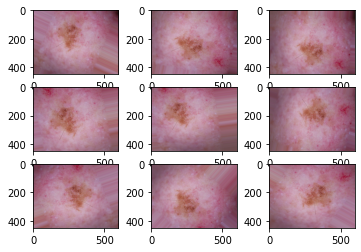
\includegraphics[width=0.5\linewidth]{./images/AnhLamGiau.png}
		\caption{Một bức ảnh khi được làm giàu bằng các tham số trên}
		\label{fig:AnhLamGiau}
	\end{figure}
	
	\subsection{Cấu trúc mạng CNN và huấn luyện mô hình}
	
	Nhưng tiêu đề của bài báo, tôi ứng dụng CNN trong việc xây dựng nên model, ảnh dưới đây thể hiện lưu đồ của mà đề tài tài này sẽ thực hiện khi có một bức ảnh hoặc một video (nhiều bức ảnh) khi đưa vào nhận diện.
	
	\begin{figure}[h!]
		\centering
		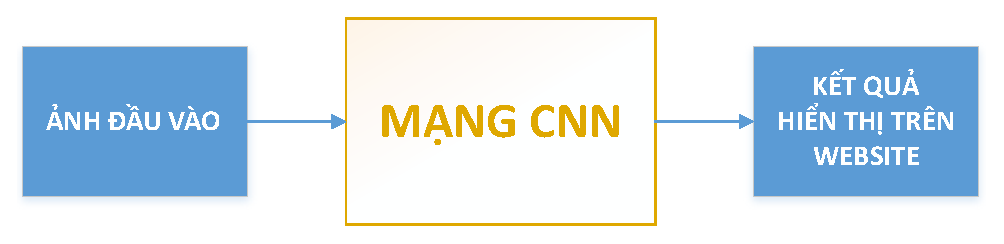
\includegraphics[width=0.8\linewidth]{./images/soDo_1.eps}
		\caption{Lưu đồ nhận diện một bức ảnh mới.}
		\label{fig:soDo1}
	\end{figure}

	\noindent
	Ở đây bức ảnh hoặc webcam của người dùng sẽ đưa vào mạng gọi chung \textit{\textbf{Input}} - là một bức ảnh, và bức ảnh này sẽ được thay đổi kích thước thành \textbf{125x125}, tiếp theo đó Input này sẽ được đưa vào các lớp trong mạng CNN và cuối cùng sẽ được đi vào các lớp ANN - các lớp được kết nối đầy đủ (Fully connected layer). Xác suất đầu ra cho tất cả các lớp sẽ được tính bằng hàm \textbf{Softmax} và lớp có xác suất cao nhất sẽ được hiển thị trên Website.\\
	
	\noindent
	Hình ảnh dưới đây là sơ đồ mạng Neural Network được tôi xây dựng:
	\begin{figure}[h!]
		\centering
		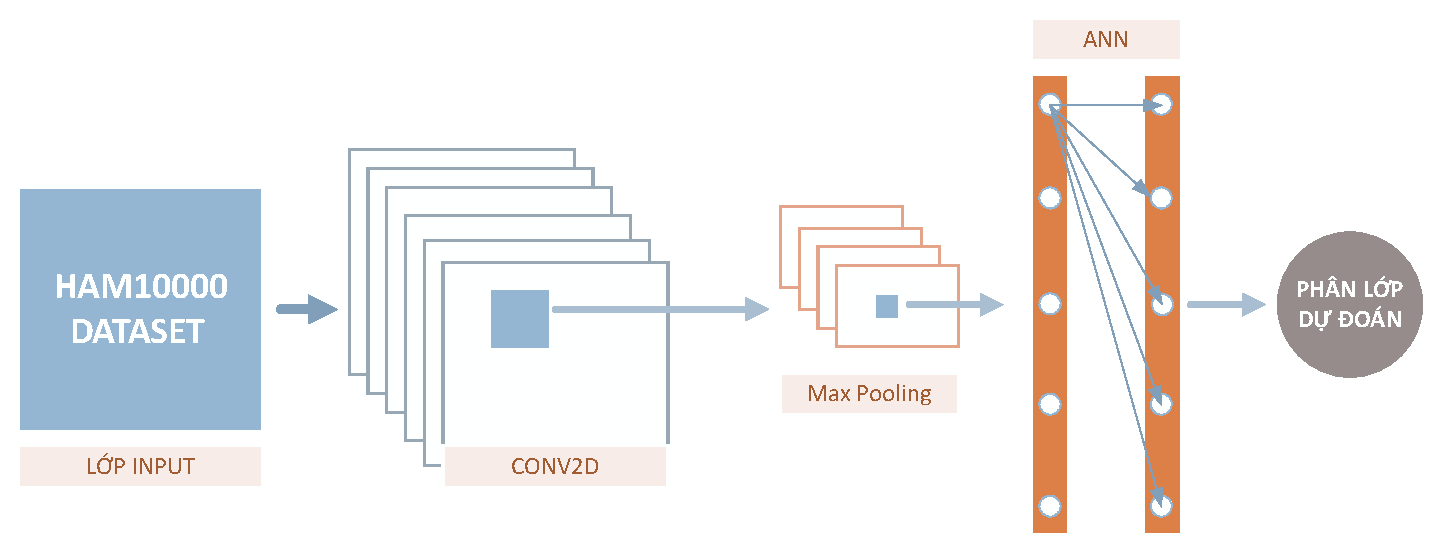
\includegraphics[width=\linewidth]{./images/SoDoCNN.eps}
		\caption{Sơ đồ mạng của đề tài.}
		\label{fig:soDoMang}
	\end{figure}
	
	\noindent
	Với cấu trúc mạng trên tôi đã sử dụng ... lớp tích chập ...\\
	
	\noindent
	Về huấn luyện (training) mô hình tôi chia tập dữ liệu HAM10000 ra theo tỉ lệ 80:20 với 80\% dùng cho traing và 20\% dùng cho testing và trong đó 15\% của dữ liệu training được dùng cho việc Validation. Với kích thước ảnh đầu vào là \textbf{125x125} và các nhãn được tôi dùng hàm \textbf{to\_categorical()} để đưa về dạng \textbf{One Hot Encoder} thích hợp trong việc huấn luyện mô hình về phân loại nhiều lớp cụ thể ở đây là 7 lớp.\\
	
	\noindent
	Với hàm mất mát (\textbf{loss funtion}) tôi lựa chọn sử dụng hàm \textbf{Categorial crossentroy} rất thích hợp khi trước đó tôi đã One Hot Encoder nhãn cùng với đây là bài toán phân loại. Cùng với đó đối với hàm tối ưu (\textbf{optimers}) tôi lựa chọn sử dùng hàm \textbf{Adams} với \textit{learning rate} khởi tạo ban đầu là 0.001.
	
	\subsection{Công cụ đánh giá mô hình}
	Có nhiều cách cũng như nhiều công cụ hay thuật toán dùng để đánh giá hiệu suất cũng như chất lương của mô hình đó. Ở đề tài nay tôi sử dụng những công cụ đánh giá rất phổ biến như: \textit{accuracy}, \textit{precision}, \textit{recall}, \textit{F1-Score}.\\
	
	\noindent
	Accuracy (Độ chính xác): Độ chính ở đây biểu thị phần trăm lớp bệnh ung thư được phân loại chính xác, được tính bằng công thức dưới đây.
	
	\begin{equation}
		accuracy = \frac{TP + TN}{TP + TN + FP + FN}\times 100
	\end{equation}

	\noindent
	Precision: Được hiểu là phần trăm lớp bệnh ung thư dương tính thật (true positive) được nhận diện chính xác.
	
	\begin{equation}
		precision = \frac{TP}{TP + FP}\times 100
	\end{equation}

	\noindent
	Recall: Các điểm dương tính thật trong tất cả các dự đoán có thể là dương tính.
	
	\begin{equation}
		recall = \frac{TP}{TP + FN}\times 100
	\end{equation}

	\noindent
	F1-Score: Là sự đánh giá dựa trên cả Precision và Recall.
	
	\begin{equation}
		F1-Score = 2\times\frac{precision\times recall}{precision + recall}
	\end{equation}
	
	\subsection{Triển khai mô hình realtime lên website}
	Triển khai mô hình (model) realtime lên website nhầm tạo ra điều kiện thuận lợi hơn với người sử dụng. Có rất nhiều sự lựa chọn Framework cũng như những ngôn ngữ Backend khác để xây dựng Webserver, với tôi thì do từng trải qua nhiều dự án với Flask Framework nên trong đề tài này tôi cũng sử dụng Flask kết hợp cùng với TensorflowJS một thư viện Javascript của chính chủ Google dành cho những lập trình viên muốn triển khai mô hình Tensorflow lên website.\\
	
	\noindent
	Cấu trúc Website được tôi thiết kế với 3 chức năng chính: nhận diện realtime sử dụng Webcam hoặc camera, nhận diện thông qua ảnh nội soi tĩnh và chức năng còn lại là trang thông tin về các loại bệnh.\\
	
	\noindent
	Nói về việc sử dụng dụng TensorflowJS, như trình bày ở phần 2.3 - Input đầu vào là một bức ảnh hoặc một video cụ thể là ảnh được lấy từ webcam hoặc ảnh từ người dùng tải lên. Với bức ảnh này sẽ được đưa về kích thước 125x125 theo chuẩn Tensor và đưa vào mô hình để nhận diện. Mô hình sẽ trả về xác suất của 7 lớp.
	
	\noindent
	Đọc giả có thể xem tham khảo Source code tôi viết qua QR Code đường dẫn Github mà tôi gắn ở trang đầu bài báo.
	%%%%%%%%%%%%%%%%%%%%%%%%%%%%%%%%%%%%%%%%%%%%%%%
	
	\section{Kết quả}
	
	%%%%%%%%%%%%%%%%%%%%%%%%%%%%%%%%%%%%%%%%%%%%%%%
	
	\section{Kết luận}
	Qua những kết quả trên tôi đưa ra kết luận cho bài báo này như sau, về cơ bản tôi đã xây dựng được mô hình sử dụng các lớp mạng CNN để phân loại mô hình, với tôi là một người chưa có nhiều kinh nghiệm vì thế mạng tôi xây dựng ra chưa đạt kết quả như mong đợi. Nếu có cơ hội được cải tiến đề tài này tôi có thể sử dụng một vài mạng được pretrained để nhằm mục đích trích xuất các đặc trưng của hình ảnh tốt hơn và cho kết quả nhận diện tốt hơn hiện tại.\\
	
	\noindent
	Bên cạnh đó tôi đã triển khai được hệ thống nhận diện lâm sàng trực tuyến thông qua Website tại địa chỉ: \href{https://skincancer.svute.com}{https://skincancer.svute.com} tuy kết quả mô hình chưa được tốt nhưng sản phẩm có thể sử dụng ở mức độ tham khảo.
\end{document}